\documentclass[fleqn]{article}
\oddsidemargin 0.0in
\textwidth 6.0in
\thispagestyle{empty}
\usepackage{import}
\usepackage{amsmath}
\usepackage{graphicx}
\usepackage{flexisym}
\usepackage{calligra}
\usepackage{amssymb}
\usepackage{bigints} 
\usepackage[english]{babel}
\usepackage[utf8x]{inputenc}
\usepackage{float}
\usepackage[colorinlistoftodos]{todonotes}


\DeclareMathAlphabet{\mathcalligra}{T1}{calligra}{m}{n}
\DeclareFontShape{T1}{calligra}{m}{n}{<->s*[2.2]callig15}{}
\newcommand{\scriptr}{\mathcalligra{r}\,}
\newcommand{\boldscriptr}{\pmb{\mathcalligra{r}}\,}

\definecolor{hwColor}{HTML}{691F80}

\begin{document}

  \begin{titlepage}

    \newcommand{\HRule}{\rule{\linewidth}{0.5mm}}

    \center

    \begin{center}
      
\includegraphics[height=11cm, width=11cm]{asu.png}
    \end{center}

    \vline

    \textsc{\LARGE Classical Parts/Field/Matter III}\\[1.5cm]

    \HRule \\[0.5cm]
    { \huge \bfseries Homework One}\\[0.4cm] 
    \HRule \\[1.0cm]

    \textbf{Behnam Amiri}

    \bigbreak

    \textbf{Prof: Samuel Teitelbaum}

    \bigbreak

    \textbf{{\large \today}\\[2cm]}

    \vfill

  \end{titlepage}

  \begin{enumerate}
    \item \textbf{(8.2. 15 pts)} Consider the charging capacitor in Prob. 7.34
    \begin{enumerate}
      \item Find the electric and magnetic fields in the gap, as functions of the distance $s$
      from the axis and the time $t$. (Assume the charge is zero at $t=0$.)

        \textcolor{hwColor}{
          \\
          Consider the charging capacitor below (Prob. 7.34)
        }

        \begin{center}
          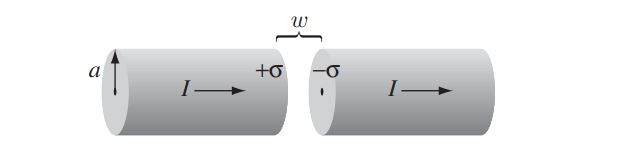
\includegraphics[height=3cm, width=10cm]{problem734.JPG}
        \end{center}

        \textcolor{hwColor}{
          Think of a single sheet that has a positive charge distributed through its surface and 
          consider a Gaussian surface in the form of a cylinder right in the middle of the sheet. Gaussian cylinder
          is going to emit an electric field that exists the cylinder in both directions. (Outward flux)
          We can calculate the electric field using the Gauss'a law: 
          \\
          \\
          $
            \bigoint E.da=\dfrac{1}{\epsilon_0} Q_{enc}
          $
          \\
          \\
          The Total electric flux for both siders of the Gaussian cylinder is $EA$. Therefore, $EA+EA=\dfrac{1}{\epsilon_0} Q$.
          We also know that surface charge density is $\sigma=\dfrac{Q}{A}$, so we have:
          \\
          $
            2EA=\dfrac{1}{\epsilon_0} \sigma A \Longrightarrow \overrightarrow{E}=\dfrac{\sigma}{2 \epsilon_0} \hat{z}
          $
          ~~~~~~ (Assuming the $\hat{z}$ is to the right)
          \\
          \\
          We now know the electric field of one plate then the electric field in between the two plates is:
          \\
          \\
          $
            \overrightarrow{E}+\overrightarrow{E}=\dfrac{\sigma}{2 \epsilon_0} \hat{z}+\dfrac{\sigma}{2 \epsilon_0} \hat{z}
            \\
            \\
            \\
            \therefore ~~~ \overrightarrow{E}=\dfrac{\sigma}{\epsilon_0} \hat{z}
          $
          \\
          \\
          Note: We assumed the charged is distributed uniformly. For a circular plate we have:
          \\
          \\
          $
            \sigma=\dfrac{Q}{A}=\dfrac{I ~ t}{\pi a^2}
            \\
            \\
            \\
            \therefore ~~~ \overrightarrow{E}=\dfrac{I ~ t}{\epsilon_0 \pi a^2} \hat{z} ~~~~ \checkmark
          $
          \\
          \\
          \\
          \\
          \\
          We can use the Ampere's law to find the magnetic field in the gap at a distance $s < a$. 
          \\
          \\
          $
            \bigoint B.dl=\mu_0 I_{enc}
            \\
            \\
          $
          In chapter 7, we learned about displacement current $J_d \equiv \epsilon_0 \dfrac{\partial E}{\partial t}$.
          Through the gap the displacment is in the $z$ direction. By rewriting the Ampere's law we have:
          \\
          \\
          $
            \bigoint B.dl=\mu_0 I_{dis} \Longrightarrow B \times 2 \pi s=\mu_0 I_{dis}
            \\
            \\
            I_{dis}=\bigints J_d.da
            =\bigints \left(\epsilon_0 \dfrac{\partial E}{\partial t}\right).da
            =\bigints\limits_{0}^{s} \bigints\limits_{0}^{2 \pi} \left[
              \epsilon_0 \dfrac{\partial}{\partial t} \left(\dfrac{I ~ t}{\epsilon_0 \pi a^2} \hat{z} \right)
            \right].s ~ ds ~ d\phi ~ \hat{z}
            \\
            \\
            =\bigints\limits_{0}^{s} \bigints\limits_{0}^{2 \pi} \left( 
              \dfrac{\epsilon_0 ~ I}{\epsilon_0 \pi a^2} \hat{z} 
            \right).s ~ ds ~ d\phi ~ \hat{z}
            =\left[\dfrac{I ~ s^2}{2 \pi a^2}\right]_{0}^{s} \times \left[2 \pi\right]
            \\
            \\
            \\
            \therefore ~~~ I_{dis}=\dfrac{I ~ s^2}{a^2} \Longrightarrow B \times 2 \pi s=\mu_0 I_{dis}=\mu_0 \dfrac{I ~ s^2}{a^2}
            \\
            \\
            \\
            \therefore ~~~ \overrightarrow{B}=\mu_0 \dfrac{I ~ s}{2 \pi a^2} \hat{\phi} ~~~~ \checkmark
          $
        }

      \item Find the energy density $u_{em}$ and the Poynting vector $S$ in the gap. Note especially 
      the direction of $S$. Check that $Eq. 8.12$ is satisfied.

        \textcolor{hwColor}{
          \\
          Eq 8.5 gives the total energy stored in electromagnetic fields as
          \\
          \\
          $
            u_{em}=\dfrac{1}{2} \left(\epsilon_0 E^2 + \dfrac{1}{\mu_0} B^2\right)
            =\dfrac{1}{2} \left(\epsilon_0  \dfrac{I^2 ~ t^2}{\epsilon_0^2 \pi^2 a^4} + \dfrac{1}{\mu_0}  \mu_0^2 \dfrac{I^2 ~ s^2}{4 \pi^2 a^4} \right)
            =\dfrac{1}{2} \left(\dfrac{I^2 ~ t^2}{\epsilon_0 \pi^2 a^4} + \dfrac{\mu_0 I^2 ~ s^2}{4 \pi^2 a^4} \right)
            \\
            \\
            \\
            \therefore ~~~ u_{em}=\dfrac{I^2}{2\pi^2 a^4} \left(\dfrac{t^2}{\epsilon_0} + \dfrac{\mu_0 s^2}{4} \right) ~~~~ \checkmark
            \\
            \\
          $
          The Poynting vector is defined in Griffiths as
          \\
          \\
          $
            \overrightarrow{S} \equiv \dfrac{1}{\mu_0} \left(E \times B\right)
            =\dfrac{1}{\mu_0} \left(
              \dfrac{I ~ t}{\epsilon_0 \pi a^2} \hat{z} 
              \times 
              \mu_0 \dfrac{I ~ s}{2 \pi a^2} \hat{\phi}
            \right)
            \\
            \\
            \\
            \therefore ~~~ \overrightarrow{S}=-\dfrac{I^2 t s}{2 \pi^2 \epsilon_0 a^4} \hat{s} ~~~~ \checkmark
          $
          \\
          \\
          The direction of $\overrightarrow{S}$ is in the $\hat{s}$ direction. We know that the direction of Poynting vector is 
          the direction of energy flow. Hence, the energy is flowing into the gap. Now we need to check that $Eq. 8.12$ is satisfied.
          $
            \dfrac{\partial u_{em}}{\partial t}=-\nabla.S  ~~~~~ Eq. 8.12.
            \\
            \\
            \begin{cases}
              \dfrac{\partial u_{em}}{\partial t}
              =\dfrac{\partial}{\partial t} \left[\dfrac{I^2}{2\pi^2 a^4} \left(\dfrac{t^2}{\epsilon_0} + \dfrac{\mu_0 s^2}{4} \right)\right]
              =\dfrac{I^2 t}{\pi^2 a^4 \epsilon_0}
              \\
              \\
              -\nabla.S=-\dfrac{1}{s} \dfrac{\partial}{\partial s} \left(s S\right)
              =-\dfrac{1}{s} \dfrac{\partial}{\partial s} \left(-s \dfrac{I^2 t s}{2 \pi^2 \epsilon_0 a^4}\right)
              =\dfrac{I^2 t}{\pi^2 \epsilon_0 a^4}
            \end{cases} \Longrightarrow \dfrac{\partial u_{em}}{\partial t}=-\nabla.S ~~~~ \checkmark
          $
          \\
          \\
          \\
          As we just saw, $Eq. 8.12$ holds. 
        }


      \item Determine the total energy in the gap, as a function of time. Calculate the total
      power flowing into the gap, by integrating the Poynting vector over the appropriate surface. 
      Check that the power input is equal to the rate of increase of energy in the gap ($Eq. 8.9$—in 
      this case $W=0$, because there is no charge in the gap). [If you’re worried about the fringing 
      fields, do it for a volume of radius $b < a$ well inside the gap.]
      
    \end{enumerate}

    \item \textbf{(8.4. 15 pts)}
    \begin{enumerate}
      \item Consider two equal point charges $q$, separated by a distance $2a$. Construct the
      plane equidistant from the two charges. By integrating Maxwell’s stress tensor
      over this plane, determine the force of one charge on the other


      \item Do the same for charges that are opposite in sign.

      
    \end{enumerate}


    \item \textbf{(8.16. 35 pts)} A sphere of radius $R$ carries a uniform polarization $P$ and a uniform
    magnetization $M$ (not necessarily in the same direction). Find the electromagnetic momentum of this configuration.
    [Answer: $\dfrac{4}{9} \pi \mu_0 R^3 (M \times P)$]
    


    \item \textbf{(8.17. 35 pts)} Picture the electron as a uniformly charged spherical shell, with
    charge $e$ and radius $R$, spinning at angular velocity $\omega$.
    \begin{enumerate}
      \item Calculate the total energy contained in the electromagnetic fields.


      \item Calculate the total angular momentum contained in the fields.


      \item According to the Einstein formula $(E = mc^2)$, the energy in the fields should
      contribute to the mass of the electron. Lorentz and others speculated that the
      entire mass of the electron might be accounted for in this way: $U_{em} = m_e c^2$.
      Suppose, moreover, that the electron’s spin angular momentum is entirely
      attributable to the electromagnetic fields: $L_{em}=\dfrac{\hbar}{2}$. On these two 
      assumptions, determine the radius and angular velocity of the electron. What is their
      product, $\omega R$? Does this classical model make sense?
      
    \end{enumerate}


  \end{enumerate}

\end{document}
